\section{Problem 1}

\subsection{Question}
Rerun A9, Q2 but this time using LIBSVM.  If you have n categories,
you'll have to run it n times.  For example, if you're classifying music
and have the categories:\\
\\
metal, electronic, ambient, folk, hip-hop, pop\\
\\
you'll have to classify things as:\\
\\
metal / not-metal\\
electronic / not-electronic\\
ambient / not-ambient\\
\\
etc.\\
\\
Use the 500 term vectors describing each blog as the features, and
your mannally assigned classifications as the true values.  Use
10-fold cross-validation (as per slide 46, which shows 4-fold
cross-validation) and report the percentage correct for 
each of your categories.\\

\subsection{Answer}
A function for the cosine similarity was made based off the definition of the dot product. This was used with the nnestimate() function

\lstinputlisting[language=Python, caption={Python script that computes kNN based on cosine similarity}, label=listing:cluster]{q1/cluster.py}

\begin{figure}[h]
\centering
\fbox{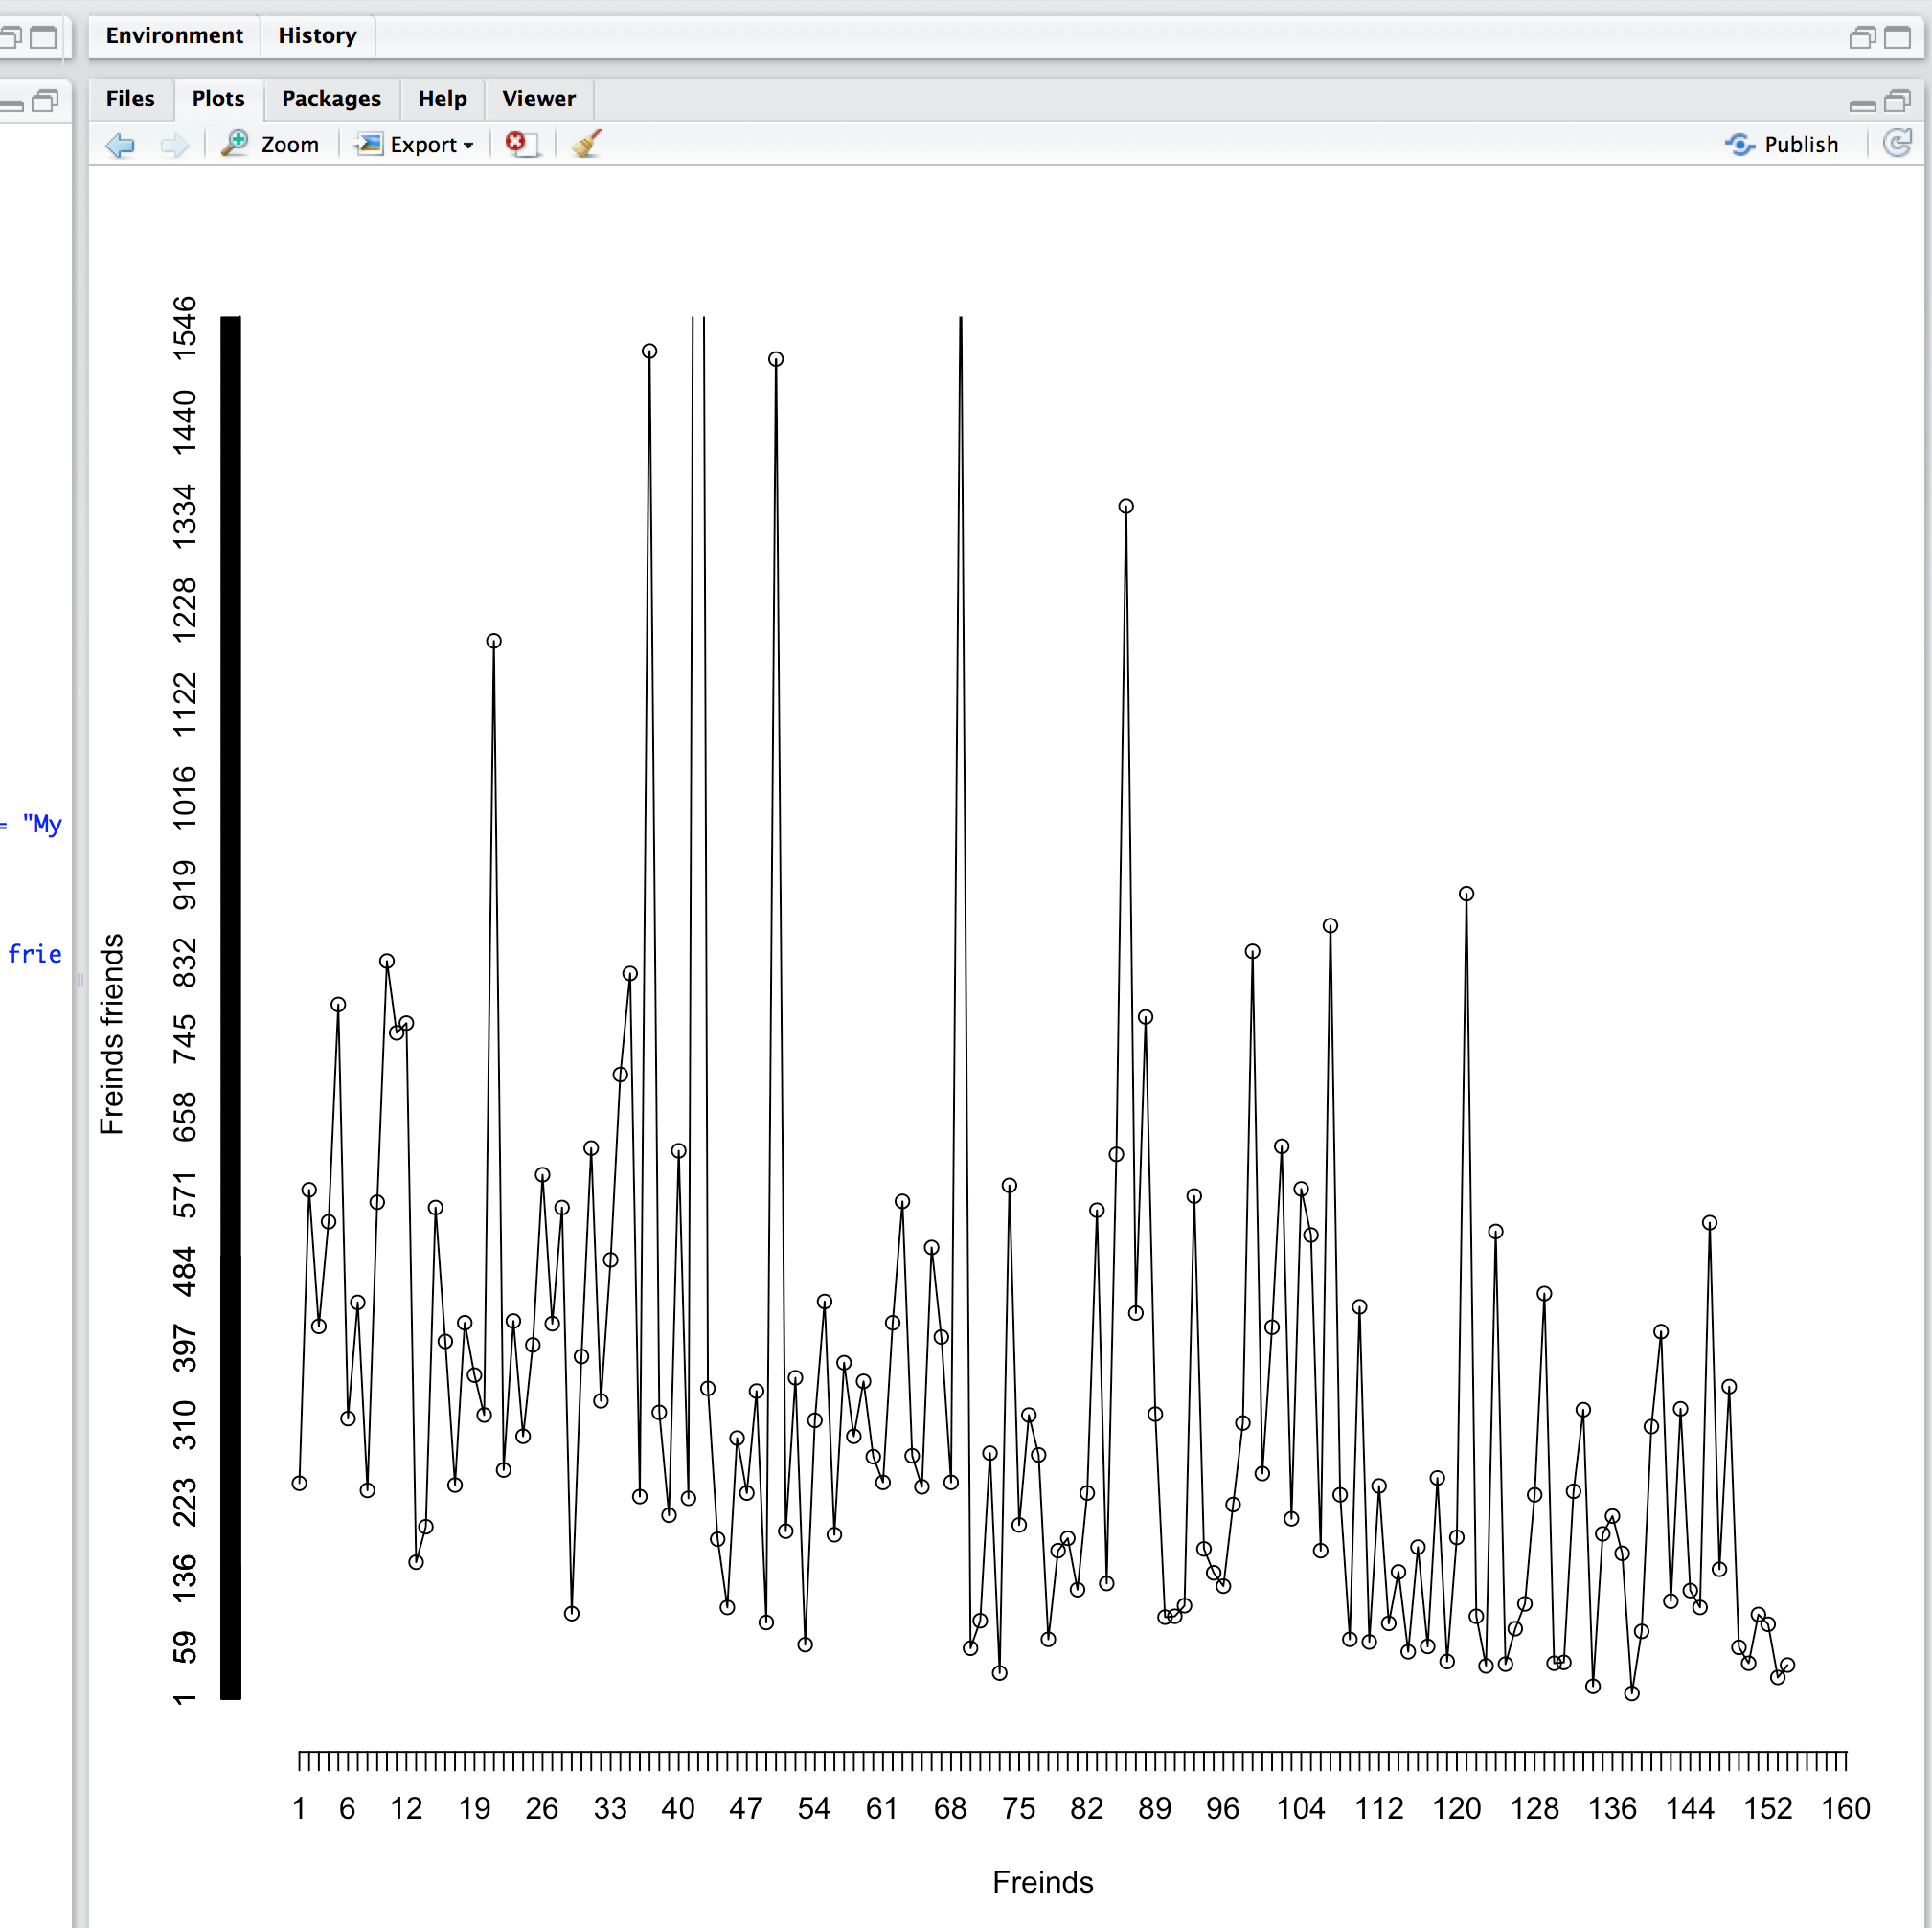
\includegraphics[scale=.85]{q1/fig1.png}}
\caption{Clustings for the F-Measure blog}
\label{fig:clust_f}
\end{figure}

\begin{figure}[h]
\centering
\fbox{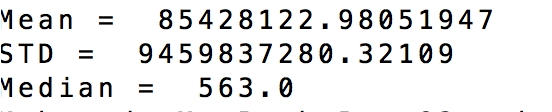
\includegraphics[scale=.85]{q1/fig2.png}}
\caption{Clusterings for the WS-DL blogs}
\label{fig:clust_ws}
\end{figure}
